\documentclass{report}
\usepackage[english]{babel}
\usepackage[utf8]{inputenc}
\usepackage[T1]{fontenc}
\usepackage{listings}
\usepackage{titlesec}
\usepackage{color}
\usepackage{graphicx}

\titleformat{\chapter}[display]
            {\normalfont\bfseries}{}{0pt}{\Huge}

\lstset{ escapeinside={(*}{*)} }

\title{Méthodes et Outils pour la Conception Avancée}
\author{Castel Antonin, Reboul Paul, Vandendorpe Thomas}
\begin{document}
\maketitle{}
\tableofcontents

\chapter{Introduction}

Ce dossier rassemble les travaux effectués lors du cours de ``Méthodes et Outils pour la Conception Avancée''. L'objectif ici, est de montrer les bonnes pratiques à avoir lors de la conception d'un programme. Nous illustrerons ces bonnes pratiques à partir de l'exemple d'un programme de puissance 4 (en langage C), initialement codé de façon peu rigoureuse, que nous tenterons d'améliorer tout au long de ce dossier. Par améliorer, on entend  la maintenabilité, la réutilisabilité et la documentation du code, la qualité et la couverture des tests, la détection de défauts et d'erreurs, l'analyse et l'amélioration des performances, ainsi que l'analyse de la vulnérabilité à certaines attaques. Nous expliquerons les différentes méthodes et outils permettants ces améliorations...

\chapter{Modularité, maintenabilité, réutilisabilité}
\section{Titre}
...
\section{Titre}
...

\chapter{Qualité des tests}
On ne peut pas parler de qualité du logiciel sans parler des tests. Bien que ne prouvant pas l'absence de bug dans un code, les tests exécutés sur un programme sont de bons indicateurs sur sa qualité. Il est nécessaire de ``penser tests'' tôt dans la création d'un logiciel, car les tests sont écrits au fur et à mesure de la conception et sont destinés à être exécutés plusieurs fois, ceci afin de vérifier que les modifications et ajouts dans le code permettent toujours de valider les tests précédents. Et ceci est d'autant plus vrai lors d'un projet en équipe où les modifications des uns peuvent affecter les modifications des autres. Nous allons dans cette partie présenter deux méthodes permettant d'assurer une certaine rigueur dans les tests: l'une au sujet des tests unitaires et la seconde concernant l'analyse de couverture.
\section{Les tests unitaires}
Les tests unitaires sont des tests s'appliquant à une partie d'un programme et permettant de vérifier le programme par bloc. Un bloc de programme est en faite une fonction, et l'idée est d'écrire un test qui appelle une certaine fonction avec certains paramètres (judicieusement choisis si possible, c'est à dire couvrant le plus de branches possibles) et de vérifier que le résultat renvoyé par la fonction est bien le résultat attendu. Il est possible d'écrire ces tests en suivant un processus de développement dirigé par les tests, qui consiste à écrire les tests avant d'écrire la fonction correspondante. Mais on peut également les écrire si on dispose déjà de la fonction à tester en utilisant sa spécification (qui devrait être facilement accessible si le code a été documenté avec un outil adéquat), ce qui arrive si l'on est amener à retoucher un code existant.

TODO: Nécessiter de prendre en compte/modifier des fonctions pour permettre le test unitaire (valeur retour etc...) + decoupage code en fonction
\subsection{Exemple de test}
Illustrons ce principe de tests unitaire à l'aide d'un exemple tiré d'un programme de puissance 4 (en langage C). Nous souhaitons écrire un test pour la fonction suivante:

\begin{scriptsize}
\begin{lstlisting}

int checkfull(Board board);

/*
*Verifie si une grille(Board) est pleine
*
*Parameters
*   board: une table de jeu
*
*Returns
*   0 si la grille est pleine, 1 sinon
*/


\end{lstlisting}
\end{scriptsize}

Il existe de nombreux frameworks permettant l'automatisation des tests unitaires, dans cet exemple, on utilise CuTest. Il peut être intéressant de remarquer (en gras) l'assignation des variable actual (valeur renvoyé par la fonction testée), de  expected (valeur attendue) et leur comparaison (qui fonctionne un peu comme une assertion).
\begin{scriptsize}
\begin{lstlisting}

void Test_checkfull(CuTest *tc){
  int i,j,expected,actual;
  Board b=boardVide(15,22);
  for(i=0;i<b.height;i++){
    for(j=1;j<=b.width;j++){
      (*\bfseries actual = checkfull(b);*)
      (*\bfseries expected = 1;*)
      (*\bfseries CuAssertIntEquals(tc, expected, actual);*)
      board_put(&b,j);
    }
  }
   (*\bfseries actual = checkfull(b); *)
   (*\bfseries expected = 0; *)
   (*\bfseries CuAssertIntEquals(tc, expected, actual); *)
}

\end{lstlisting}
\end{scriptsize}

Les tests écrits de cet façon pourrons ensuite tous être exécuter en même temps et des informations sur les échecs des tests seront disponibles:


\begin{lstlisting}

.......F.........

There was 1 failure:
1) Test_checkfull: src/CuTestTest.c:221: expected <0> but was <1>

!!!FAILURES!!!
Runs: 17 Passes: 16 Fails: 1

\end{lstlisting}
\begin{lstlisting}

.................

OK (17 tests)
\end{lstlisting}

Comme les tests sont ensuite facile à relancer, il est important de les réexécuter à chaque changement important dans le code afin d'évité la régression.

\subsection{Couverture}
La couverture est un indicateur permettant de savoir quelles parties du code ont été couvertes par les tests. Utiliser la couverture seule n'est pas forcément intéressant, puisqu'elle n'indique pas si les tests ont été validés ou non. En revanche, en combinaison des tests unitaire vu précédemment, on a un indicateur de la qualité des tests très puissant puisqu'on a l'information du pourcentage du code tester et du nombre de tests validés.
\subsection{Exemple de couverture}
Nous avons utilisé l'outil gcov afin d'observer la couverture de notre puissance 4. Comme ce dernier ne donne qu'un résultat textuel de la couverture, nous avons complété son utlisation avec l'outil lcov, qui utilise ce que gcov a produit mais rajoute une interface html afin que la couverture soit plus facile à lire. On peut ainsi observer le pourcentage de lignes/fonctions visitées par les tests:

En plus des pourcentage de couverture, on peut également directement voir sur le code ce qui a été couvert(en bleu) et ce qui ne l'a pas été(en rouge). Cela est pratique lorsqu'on écrit des tests en essayant de passer par le plus de branches possibles (conditions,boucles,...) du programme.

\newpage
\chapter{Analyse de performance}
\section{Outil pour l'analyse de performance}
Au dela de l'aspect programmation, qui se doit d'être affiné le plus possible afin que le programme s’exécute dans un temps minimal, nous avons optimisé le programme afin de minimiser les temps d'accès aux caches du processeur.
En effet, une erreur de prédiction de saut ou une donnée non présente dans un cache lors de l’accès fait perdre un temps considérable dans l'exécution du programme, car il faut dans un cas detecter l'erreur de branchement et la corriger, et dans l'autre c
as aller chercher la donnée dans la mémoire.
Pour optimiser cet aspect, nous avons principalement fait deux choses : 
\newline
- Nous avons remplacé les séries de "if" par des "switch", car la table de branchement de ce dernier minimise le pourcentage de "branch miss". 
\newline
- Nous avons changé les ordres de parcours des tableaux dans la mesure du possible afin de minimiser cette fois le pourcentage de "cache miss".
\newline
Bien que les résultats sur un programme qui s’exécute aussi vite que notre puissance 4 ne soit pas vraiment visibles, nous avons pu réduire grandement le nombre de "cache miss" et de "branch miss".

Sur un projet de plus grande envergure, optimiser cet aspect est essentiel.
Nous avons travaillé avec l'option "Cachegrind" de Valgrind pour détecter et dénombrer le taux de miss.

\section{Exemple d'analyse de performance}

On peut voir sur le tableau suivant un certain nombre d'informations qui représentent le pourcentage de miss des différents caches, ainsi que le nombre concret de miss. 
Nous pouvons aussi voir le pourcentage de "branch miss" dans les dernières lignes. 
Ce tableau est extrait d'une exécution de Cachegrind sur la version de base du projet, avant toute modification (hormis celles qui permettent simplement au programme de compiler).
Ce tableau se comprend comme ceci :
\newline
I fait référence au cache instruction, I1 au cache le plus rapide d'accès et LL (pour "last level") aux caches plus éloignés.
\newline
D fait référence au cache de données (Data) et fonctionne sur le même principe.
Les branchements quant à eux sont simplement énoncés à la fin de l'analyse.

\begin{scriptsize}
\begin{lstlisting}
==4891== 
==4891== I   refs:      4,320,762
==4891== I1  misses:       14,181
==4891== LLi misses:        1,990
==4891== I1  miss rate:      0.33%
==4891== LLi miss rate:      0.05%
==4891== 
==4891== D   refs:      1,758,266  (1,140,077 rd   + 618,189 wr)
==4891== D1  misses:        3,357  (    2,709 rd   +     648 wr)
==4891== LLd misses:        2,668  (    2,086 rd   +     582 wr)
==4891== D1  miss rate:       0.2% (      0.2%     +     0.1%  )
==4891== LLd miss rate:       0.2% (      0.2%     +     0.1%  )
==4891== 
==4891== LL refs:          17,538  (   16,890 rd   +     648 wr)
==4891== LL misses:         4,658  (    4,076 rd   +     582 wr)
==4891== LL miss rate:        0.1% (      0.1%     +     0.1%  )
==4891== 
==4891== Branches:        804,931  (  754,035 cond +  50,896 ind)
==4891== Mispredicts:      20,138  (   19,816 cond +     322 ind)
==4891== Mispred rate:        2.5% (      2.6%     +     0.6%   )
\end{lstlisting}
\begin{center}
\textbf{\textit{Figure 1 : Execution de Cachegrind sur le programme de base.}}
\end{center}
\end{scriptsize}

Après les modifications de notre programme, nous avons obtenu les valeurs suivantes, qui s’interprètent exactement de la même façon.
\begin{scriptsize}
\begin{lstlisting}
==5578== 
==5578== I   refs:      5,222,873
==5578== I1  misses:        2,457
==5578== LLi misses:        1,762
==5578== I1  miss rate:      0.05%
==5578== LLi miss rate:      0.03%
==5578== 
==5578== D   refs:      2,167,133  (1,304,576 rd   + 862,557 wr)
==5578== D1  misses:        6,828  (    4,225 rd   +   2,603 wr)
==5578== LLd misses:        4,814  (    2,422 rd   +   2,392 wr)
==5578== D1  miss rate:       0.3% (      0.3%     +     0.3%  )
==5578== LLd miss rate:       0.2% (      0.2%     +     0.3%  )
==5578== 
==5578== LL refs:           9,285  (    6,682 rd   +   2,603 wr)
==5578== LL misses:         6,576  (    4,184 rd   +   2,392 wr)
==5578== LL miss rate:        0.1% (      0.1%     +     0.3%  )
==5578== 
==5578== Branches:      1,073,634  (1,001,931 cond +  71,703 ind)
==5578== Mispredicts:      24,986  (   22,529 cond +   2,447 ind)
==5578== Mispred rate:        2.3% (      2.5%     +     3.4%   )
\end{lstlisting}
\begin{center}
\textbf{\textit{Figure 2 : Exécution de Cachegrind sur le programme modifié.}}
\end{center}

Comme on peut le voir, le nombre de "cache miss" à grandement diminué vu que nous sommes passés de 0.33\% à 0.05\%. 
\newline
Il serait probablement possible d'améliorer encore ce score mais cela demanderais beaucoup de temps car cela nécessiterait de reprendre un grand pourcentage du code, ce qui ne vaut pas forcement le coup étant donné que 0.05\% de miss est un score correct.
\newline
Pour ce qui est des prédictions de branchements, elles ont très peu diminuées car les améliorations que nous avons faites sont peu nombreuses, le programme ne ce porte pas vraiment à ce genre d'optimisation.
\newline
Il est à noter qu'il est normal d'avoir quelques "branch miss" sur un programme de cette taille.
\end{scriptsize}

\newpage
\chapter{Analyse de vulnérabilité }
\section{Outil pour l'analyse de vulnérabilité}
Nous avons déjà vu précédemment l'outil KLEE, qui permet de détecter des erreurs automatiquement dans un programme en simulant des traces d’exécution de ce dernier, en essayant d'avoir la plus large couverture de code possible. 
\newline 
Dans ce même but, nous avons utilisé l'outil AFL qui va lui aussi détecter des erreurs via une analyse statique. AFL va, contrairement à KLEE qui modifie directement les variables dans le code, modifier un fichier d'entrées donné par l'utilisateur.
\newline
Ce fichier, qui doit couvrir une partie des entrées possible du fichier, va ensuite être transformé par AFL pour trouver des plantages.
\newline
La modification est dite "génétique" dans le sens où, même si les modifications sont aléatoires, une modification utile (qui provoque un plantage) sera repérée et alors les transformations suivante du fichier iront dans le même sens, pour provoquer d'autres potentiels plantages.
\newline
Chaque plantage est alors une potentielle faille de sécurité à corriger.
Les bugs trouvés sont donc en grande partie des entrées incorrectes. 
\newline
Les fichiers d'entrées provoquant un plantage sont alors sauvegardés et transmis à l'utilisateur qui peut alors corriger les bugs.

\section{Exemple d'analyse de vulnérabilité}
Dans notre puissance 4, l'une des choses lue par le programme est le fichier XML qui donne la taille de la grille.
Bien que ce soit potentiellement intéressant de trouver des bugs dans la lecture de ce fichier, nous avons préféré nous focaliser sur le fuzzing des entrées des joueurs du programme.
Nous avons donc fait le nécessaire pour que afl prenne ce fichier en paramètre.
Nous allons maintenant voir un exemple de l'exécution d'AFL sur le projet de base.
Nous pouvons trouver un grand nombre d'informations, et principalement le nombre de crash, crash unique, les chemins empruntés et les timeout.

\begin{center}
  %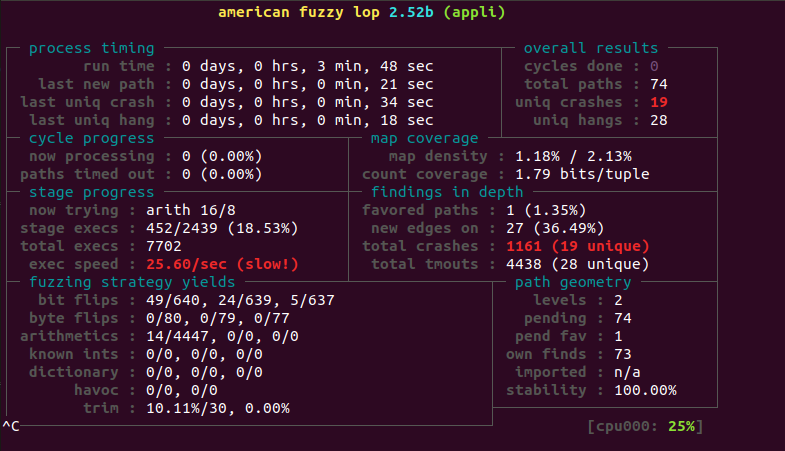
\includegraphics[width=13cm]{captureafl1.png}
\textbf{\textit{Figure 1 : Exécution d'AFL sur le programme de base.}}
\end{center}

Nous pouvons voir un très grand nombre de crashs uniques, voici maintenant l'éxécution d'AFL sur le projet modifié : 

\begin{center}
  %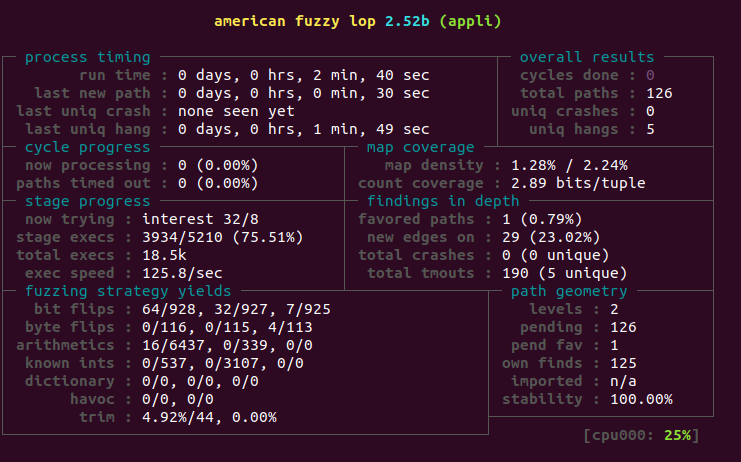
\includegraphics[width=13cm]{captureafl2.png}
\textbf{\textit{Figure 2 : Exécution d'AFL sur le programme modifié.}}
\end{center}

Comme nous pouvons le constater, les crashs ont disparus grâce aux modifications que les différents outils nous ont amené à faire, nous avons résolu certains bug avec AFL mais comme malheureusement il ne peut détecter que les crashs, son utilisation doit se faire en complementarité avec d'autres outils comme Valgrind.




\end{document}





















